\chapter{Performance Analysis}

This section presents performance characteristics of our algorithm measured through simulations using JBOTSIM\cite{26} tool. We consider the following metrics defined for any component of size $n$.

\begin{enumerate}
\item \textbf{Latency} $l$. The number of rounds necessary for a component to elect a leader (become stable) after a topology change (average over all initial topologies).

\item \textbf{Sensitivity} $s$. The number of nodes that updated their heights in response to a topology change (average over all possible topology changes).

\item \textbf{Resilience} $r$. The maximal fraction of links which can go down in a stable component without reelecting the current leader.

\end{enumerate}

We have measured these parameters using simulations of several scenarios (Figures 6(a) and 6(b)), and we summarize them below:

\begin{itemize}
\item Merging two stable components:

\begin{itemize}
\item Given two fully connected (every two nodes are neighbours) components: $l \simeq 2$.
\item Given two poorly connected (a node can have not more than two neighbours) components: $l \simeq n$.
\end{itemize}

\item Partitioning a stable component:

\begin{itemize}
\item Getting two fully connected component: $l = 2$.
\item Getting two poorly connected component: $l = 2n$.
\end{itemize}

\item Topology change in a “small world-like” stable component (every node has O(log n) neighbours) without partitioning:
\begin{itemize}
\item Latency $l$ = $O(1)$.
\item Sensitivity $s$ = $O(log(n))$.
\end{itemize}

\item Resilience of a stable component:

\begin{itemize}
\item Given a fully connected component: $r \approx 1 - 2/n$.
\item Given a “small world-like” component: $r \approx 1 - 2/log(n)$.
\end{itemize}

\end{itemize}


\begin{figure}[hbtp]
\centering
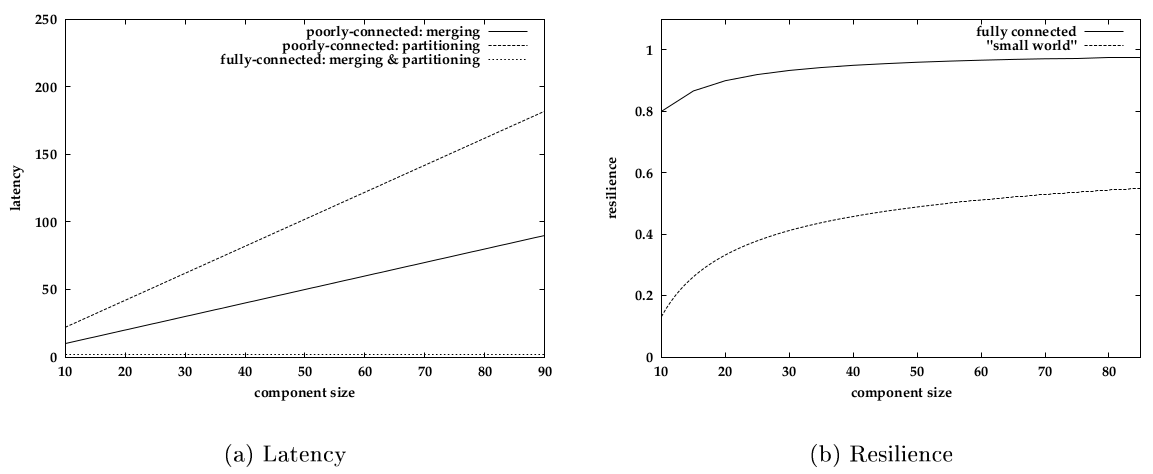
\includegraphics[scale=.4]{performance_test.png}
\caption{Simulation results}
\end{figure}